%% ============================================================================
%% pnas_draft.tex — PNAS research article, DRAFT v3 (after the round-4 referees)
%% Claude Opus 5.5 (Anthropic), Claude Code, 2026-10-19. Owner decisions: MODEL_STATUS §2z-dg §6, §2z-dh §§8-10.
%% v3 changes (SYNTHESIS_R4.md; record §2z-dj): the answer leads (the balance of volatility and decline, shown by
%% 30-year counterfactuals; durability as a separation of time scales); flattening is c/s = S*/S, not a discovery;
%% the top turns over fastest because the head is flattest (calibrated worlds at 20 seeds), not because of
%% size-blindness; the raw size exponent is uninformative, the lasting one weaker than firms'; the head's fall is
%% in participation (exact split), not asserted to be caused by persistence; named Reddit communities (owner).
%% Every number cites its record section in a comment. Development data only.
%% Compile: cd paper && pdflatex pnas_draft && bibtex pnas_draft && pdflatex pnas_draft (x2)
%% ============================================================================

\documentclass[9pt,twocolumn,twoside]{pnas-new}
\templatetype{pnasresearcharticle}
\usepackage{graphicx}
\graphicspath{{../llm_fitting/runs/2026-10-18_pnas_push/}}

%% First-page sidebar, set explicitly (2026-10-18): the repository's pnasresearcharticle.sty (v1.3, 2018) places the
%% Significance box and author information with \afterpage, which does not fire with the 2025 class's output
%% routine, so the box landed at the end of the document and body text ran into the sidebar. \Firstpage (2025
%% template) sets the wide first-page column; \FirstPageBreak, placed where that column fills, sets the sidebar
%% in the right column, ends page 1 and restores the normal column width.
\additionalelement{}
\makeatletter
\newcommand{\FirstPageBreak}{%
  {\parfillskip=0pt\par}%
  \vfill\eject
  \setlength{\columnwidth}{0.29\textwidth}\setlength{\linewidth}{0.29\textwidth}\setlength{\hsize}{0.29\textwidth}%
  \noindent\begin{minipage}[t]{150pt}\sffamily
    \mdfdefinestyle{pnassigstyle}{backgroundcolor=pnasblueback,linecolor=pnasblueback,fontcolor=pnasbluetext,innertopmargin=9.3pt,innerrightmargin=11.4pt,innerbottommargin=12pt,innerleftmargin=11.4pt,linewidth=0pt,userdefinedwidth=150pt}%
    \begin{mdframed}[style=pnassigstyle]%
      {\sffamily\bfseries\fontsize{10}{12}\selectfont\textcolor{pantone}{Significance}\par}\vskip6pt
      \raggedright\fontsize{8.5}{12}\selectfont\textcolor{black}{\@significancestatement}
    \end{mdframed}%
  \end{minipage}\par
  \vfill
  \noindent\begin{minipage}[b]{150pt}\sffamily\scriptsize
    \if!\AB@affillist!\else Author affiliations: \AB@affillist\par\vskip11.7pt
    \hrule width 150pt height.5pt\par\vskip13.5pt\fi
    \@ifundefined{@authorcontributions}{}{\@authorcontributions\par}\vskip3pt
    \@ifundefined{@authordeclaration}{}{\@authordeclaration\par}\vskip3pt
    \@ifundefined{@correspondingauthor}{}{\@correspondingauthor\par}
  \end{minipage}\par
  \vskip2pt
  \eject
  \normalcolwidth
  \noindent\ignorespaces}
\makeatother
%% let tall double-column figures sit at the top of a text page rather than alone on a float page
\renewcommand{\dbltopfraction}{0.85}\renewcommand{\dblfloatpagefraction}{0.8}\setcounter{dbltopnumber}{2}
\newcommand{\todo}[1]{\textcolor{red!65!black}{\textbf{[TODO: #1]}}}

%% Title. Owner, 2026-10-18: on the question of where the durable / quasi-stable hierarchy comes from when churn is
%% so high; framing fine. Round 4 (all three referees): "holds up" was the weakest word, since the two-year
%% counterfactuals did not show collapse without churn on comments. R6 (30-year runs from the observed ladder):
%% without churn the head's shape collapses (-61%, -90%), without the slide it steepens without limit (+28%, +67%),
%% together they hold it near the balance. "How" marks a mechanism account (PNAS precedent: "How digital media drive
%% affective polarization through partisan sorting"). Owner to confirm.
%%  USED  "How constant turnover holds up a durable hierarchy of online attention"
%%  ALT   "Why the hierarchy of online attention outlasts its members" (Opus R4)
%%  ALT   "Constant turnover sets the steepness of a durable hierarchy of online attention" (Fable R4)
%%  ALT   "How turnover replenishes a durable hierarchy of online attention" (gpt R4)
%%  earlier: "Constant turnover holds up the durable hierarchy of online attention" (v2, owner-directed question)
\title{How constant turnover holds up a durable hierarchy of online attention}

\articletype{Social Sciences (classification placeholder)}
\author[a,1]{Author One}
\affil[a]{Affiliation placeholder}
\leadauthor{One}
\authorcontributions{Placeholder.}
\authordeclaration{The authors declare no competing interest.}
\correspondingauthor{\textsuperscript{1}Placeholder.}

\significancestatement{A few communities, pages and channels hold most online attention, in a hierarchy that outlasts its members: a quarter to a third of the top ten Reddit communities are replaced every year, yet the shape of the hierarchy takes years to decades to change. Where does it come from? From random growth held in check. Volatility spreads communities apart, the relative decline of those above each rank pulls them back, and the balance of the two sets the hierarchy's steepness. Without the volatility the hierarchy would collapse; without the decline it would steepen without limit. It changes slowly because what its members lose and what newcomers bring are each small against its span. Unlike random growth, declines in participation persist.}

\keywords{attention inequality $|$ Gibrat's law $|$ rank dynamics $|$ turnover $|$ online platforms}

\begin{abstract}
Online attention is concentrated in a durable hierarchy whose members change constantly. In weekly activity of Reddit communities (2019--2022) and Facebook pages (2020--2022), 15--33\% of each Reddit top set is replaced every year, yet the hierarchy's shape changes by at most a third of a log unit a year, against a span of three to four. We ask where the hierarchy comes from. Volatility spreads communities apart and the relative decline of those above each rank pulls them back; their balance sets the hierarchy's steepness at each rank. A generative model built from the measured volatility and decline forms the hierarchy from equality within a decade; without the volatility it collapses over decades, and without the decline it steepens without limit. Measured rank by rank, crossings into each top set return lasting variance over twice the local slope (measured over predicted, 0.94; 90\% interval 0.86--1.04), about three quarters of what its members lose. Both terms are small against the hierarchy's span, which is why it outlasts its members. The top sets turn over fastest because the hierarchy is flattest at the top, and lasting volatility falls with size less steeply than for firms. Unlike random growth, participation persists: on Reddit, changes in activity are correlated (0.13--0.20) between periods that share no weeks, mostly in decline, not explained by the 2020 surge or a 2021 change in capture. The fall of the submissions head's share, from 50\% to 34\%, came through participation: its share of posts fell from 22\% to 9\%.
\end{abstract}

\dates{This manuscript was compiled on \today}

\begin{document}
\maketitle
\thispagestyle{firststyle}
\ifthenelse{\boolean{shortarticle}}{\ifthenelse{\boolean{singlecolumn}}{\abscontentformatted}{\abscontent}}{}
\Firstpage

\dropcap{A}ttention online is concentrated: on every large platform a small number of communities, pages and channels receive most of the activity, along a steep rank--size curve. Yet the occupants of that curve do not stay, and attention to individual items decays within days \cite{wu2007}. In the data we study, about one in six of the top 12,500 Reddit communities is replaced within a year, and among the top ten between a quarter and a third. The curve itself changes slowly. Where does a durable hierarchy come from when its occupants turn over so fast?
%% §2z-cu; §2z-dg A1, A7-5

Several bodies of work speak to this. Firm growth is size-dependent: the spread of a firm's annual growth falls with its size as a power with exponent near 0.2 \cite{stanley1996,amaral1997,riccaboni2008}, so large firms are steadier, and cumulative advantage lets early leaders accumulate more \cite{merton1968,salganik2006,vanderijt2014}. Online, the sizes of websites follow from multiplicative random growth \cite{huberman1999}, popularity moves in bursts \cite{ratkiewicz2010}, and the engagement of news outlets on Facebook grows independently of their size \cite{sangiorgio2024}. Studies of ranking dynamics across many systems find the occupant of the top rank the most stable \cite{iniguez2022,blumm2012}, and cities show the same coexistence of a stable rank--size law with churning membership \cite{batty2006,duranton2007}. Random-growth theory explains how such laws can be stationary despite movement: volatility spreads units apart and a drift that holds back the larger ones keeps the distribution from spreading without limit \cite{gibrat1931,champernowne1953,gabaix1999,gabaix2009,gllm2016}. Stochastic portfolio theory states the balance rank by rank---the steepness at each rank is set by the volatility there and the relative decline of the units above it---and gives estimators for it \cite{fernholz2002,banner2005,ichiba2011,fernholz2017}; Gomez's decomposition of top shares gives the same accounting for a top set, whose share changes through its members' growth and through displacement at its boundary \cite{gomez2023}, and rank-based models with entry and exit describe the balance for equity markets \cite{bakersmyth2026}.

\FirstPageBreak\indent We take these ideas to online attention and measure each ingredient rank by rank, for named communities whose week-to-week movement is mostly passing. To separate what random growth implies automatically from what it does not, we compute every statistic, with the same estimators, in the data and in simulated worlds: size-blind and firm-like random growth, started from the data's own ladder, neutral copying \cite{bentley2007}, and the model we build. Three findings follow. The hierarchy is the balance of random growth: its steepness at each rank is volatility over the relative decline of those above, the measured ingredients build it from equality and hold it against collapse, and it is durable because what its members lose and what newcomers bring are each small against its span. Its top sets turn over fastest because the hierarchy is flattest at the top, and size gives communities less of the protection it gives firms. And, unlike any random-growth world, Reddit shows persistent decline in participation.

\section*{Results}

\subsection*{A fast turnover and a durable hierarchy}
We study three ladders (\textit{Materials and Methods}): the weekly comment karma of Reddit communities and their submission karma, each from December 2018 to December 2022, and the weekly interactions of Facebook pages from November 2020 to June 2022. Each ladder is a top-$K$ universe ($K$ = 12,500 comment communities, 5,000 submission communities, 3,500 pages). In a year, 15--26\% of each Reddit top set from the top 78 to the top 6,250 is replaced, by cut-off and year, and 27--33\% of each top ten on average; on Facebook 18--35\% of each top set is replaced in half a year (Fig.~1\textit{C}). The hierarchy changes far more slowly. Its shape, $U_k - U_K$ with $U_k$ the mean log activity of the top $k$, moves by at most a third of a log unit a year at any cut-off and over any year ($-0.32$ to $+0.16$), against a span of three to four (Fig.~1\textit{A}), and on comments not in one direction: in some years the head flattened while the body steepened. Concentration fell steadily: the arithmetic share of every top set we measured fell in every year, most at the head of submissions, where the 78 leading communities' share of the top 5,000's activity fell from 50.2\% in 2019 to 34.0\% in 2022 (Fig.~5\textit{C}). The leaders mostly kept their places while losing ground. r/memes was the largest submissions community in 196 of 212 weeks while its share fell from 7.0\% to 1.8\%, and r/AskReddit the largest comments community in 209 of 213 weeks while its share fell from 11.3\% to 4.9\%; of the 2019 head of submissions, three quarters lost share, and three had left the top 5,000 by 2022, two of them banned by Reddit in June 2020.
%% turnover: out_turnover_kinematics.txt, exponent_robustness.json; shape: law cells (annual and half-year-start cells, -0.319..+0.162/yr); A8; R5 (head_named.py)

\begin{figure*}[tbp]\centering
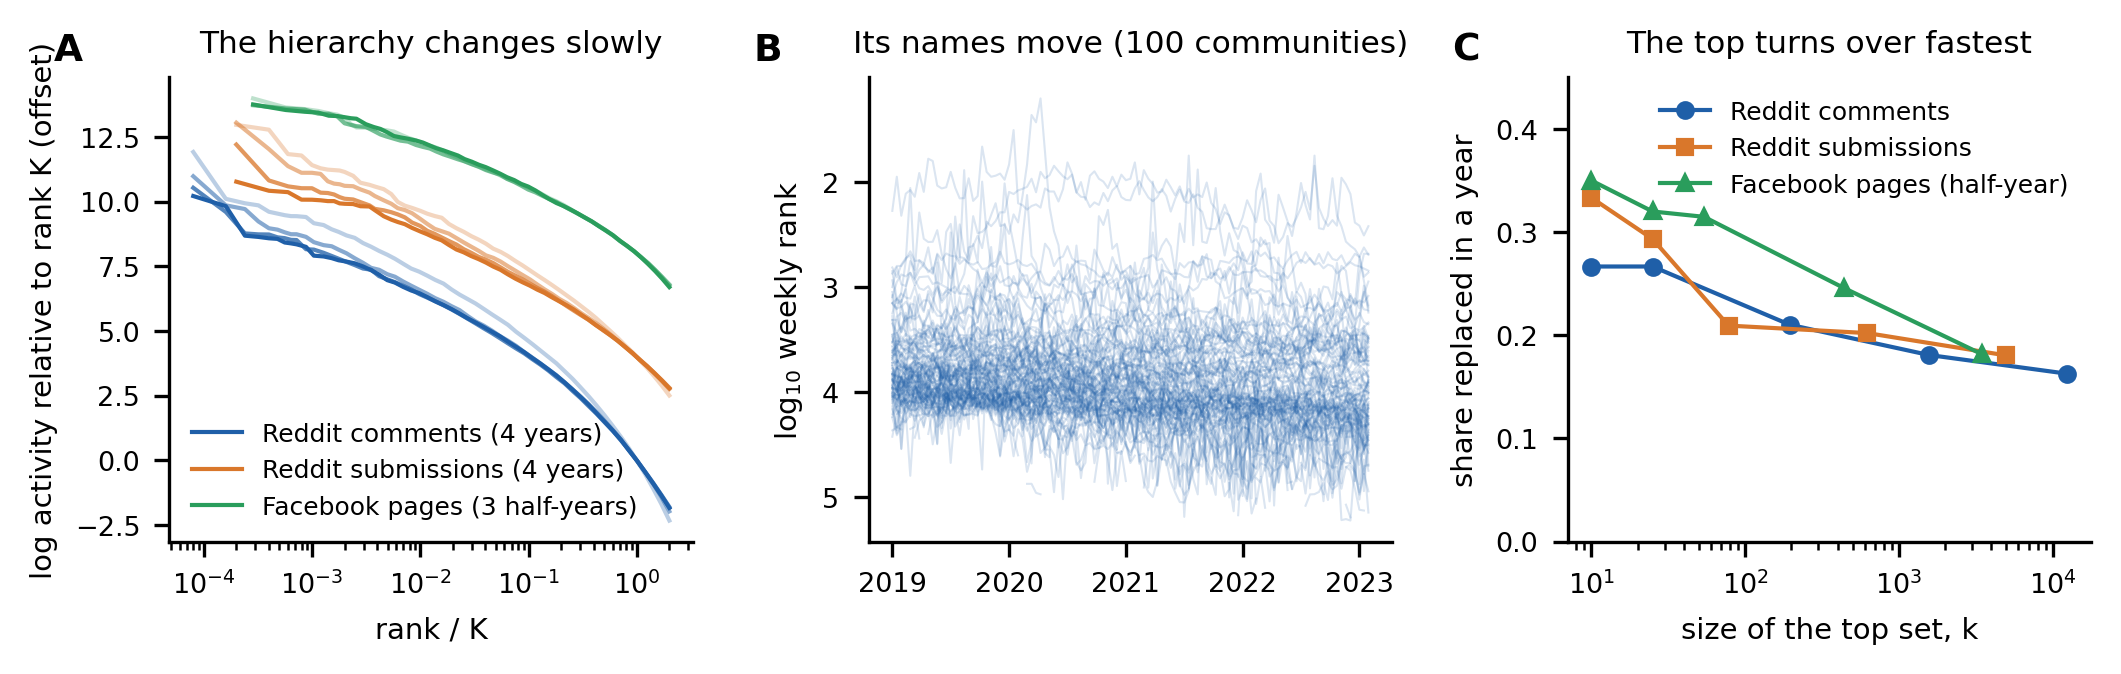
\includegraphics[width=\textwidth]{fig1_puzzle}
\caption{A fast turnover and a slowly flattening hierarchy. (\textit{A}) The rank--size curve of each ladder, one curve per year (Reddit) or half-year (Facebook), darker = later; curves offset. (\textit{B}) Weekly ranks of 100 random communities from the 2019 top 12,500 of Reddit comments. (\textit{C}) The share of the top $k$ replaced within a year (Facebook: half a year), mean over year pairs, from the top ten to the universe.}
\end{figure*}

\subsection*{The top turns over fastest because the hierarchy is flattest there}
Which top sets turn over fastest follows from the ladder's geometry. The share of a top set that leaves in a year is set by how far its members move against the local slope $S_k$ of log activity on log rank:
\begin{equation}
f_k \;=\; v_k + (1-v_k)\,\mathbb{E}\!\left[\,1 - e^{-D^{+}/S_k}\right],
\label{eq:turnover}
\end{equation}
where $D^{+}$ is the downward move of a member near the boundary relative to the boundary itself and $v_k$ the share that vanish. Eq.~\ref{eq:turnover} is kinematics: it holds in every simulated world as in the data (all 48 data cells within 0.82--1.18 of observed, median 0.98; the exact form was derived after a linear approximation failed). As a decomposition it shows where the fast turnover at the top comes from (Fig.~3\textit{C}): the typical downward move at the boundary is nearly constant across scale (0.21--0.40 log units), while the slope rises from 0.7--1.0 at the head to 1.2--2.3 lower down. Simulated worlds confirm that the order comes from the ladder (Fig.~2\textit{B}; 20 runs each). Started from the data's own ladder, the top ten turn over fastest whether volatility is independent of size (0.21 a year against 0.14 at $K/2$) or falls with size as it does for firms (0.19 against 0.14); started from a ladder of constant slope, size-blind growth turns every top set over at the same rate (0.24 against 0.23), and firm-like growth protects the top (0.13 against 0.25).

Size gives communities less protection than it gives firms, though more than none. For firms, the standard deviation of annual growth falls with size as $\mathrm{size}^{-\beta}$ with $\beta \approx 0.15$--$0.2$ \cite{stanley1996,amaral1997,riccaboni2008}. Measured the same way---communities stratified by permanent rank (their mean rank over a fixed block, absences counted at the floor), one-year changes of mean log activity---$\beta = 0.075$ (5--95\%: 0.061--0.093) and 0.059 in the following year on Reddit comments, 0.045 and 0.082 on submissions, and 0.008 on Facebook pages (Fig.~2\textit{A}). This raw exponent says little here, because passing swings that differ by rank dominate it: in the world calibrated to Reddit submissions a planted exponent of zero is measured as 0.06 and a planted 0.2 as 0.09. Estimated on the lasting part of the change by the model's structure function, which recovers a planted exponent within about 0.03 on panels of this length, the exponent is 0.05 on submissions and 0.06--0.13 on comments, depending on the window; Facebook's record is too short for that estimator, and a two-step estimate of its lasting part gives 0.02 (\textit{SI Appendix}). Day-to-day fluctuations of web traffic scale weakly with size \cite{menezes2004,eisler2008}, and the engagement of Facebook news outlets grows independently of their size \cite{sangiorgio2024}.

The occupant of a single rank is another matter. Ranking studies find the top stable by how often the occupant of a rank changes \cite{iniguez2022}, and by that measure the top of Reddit is stable too: the leading community of comments changed in 3\% of weeks and of submissions in 7\%, against more than 90\% of weeks at rank 50 (Fig.~2\textit{C}). The level gap between neighbouring ranks is about $S/R$, large at rank one, so set replacement and rank change are two statistics of one ladder. Facebook is different: its leading page changed in 52\% of weeks.
%% R7 (null_worlds_r7_summary.json: sb_data, firm_data, gibrat, atlas); rank_change_data.json (R3-B); A1; §2z-dc; recovery: runs/2026-10-18_rdm/recovery_output.txt

\begin{figure*}[tbp]\centering
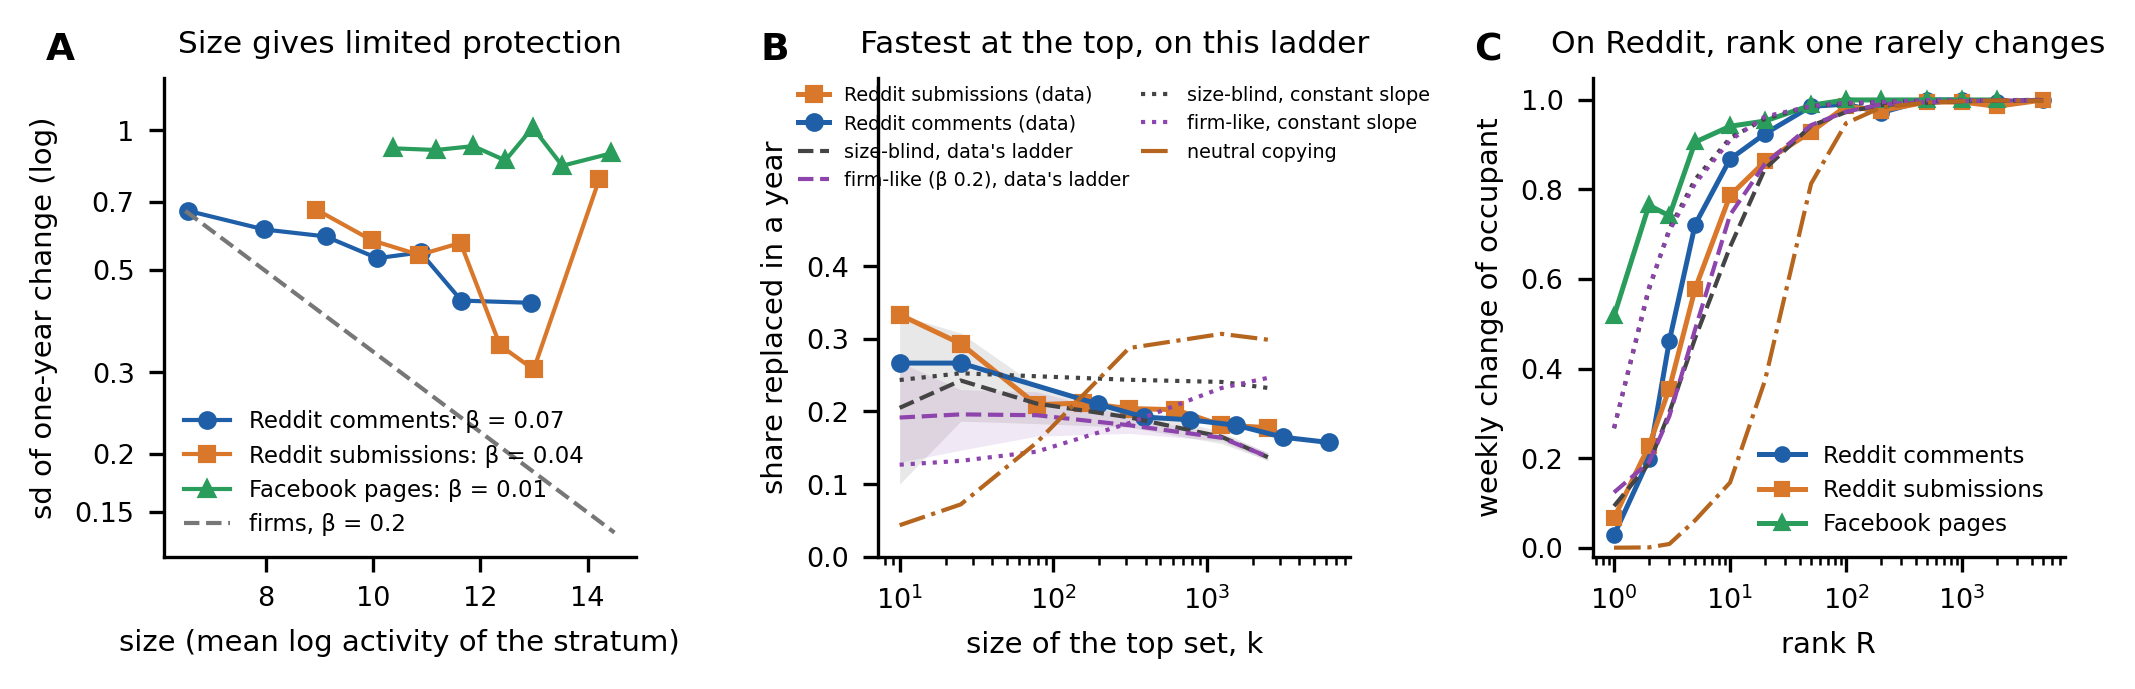
\includegraphics[width=\textwidth]{fig2_size_blind}
\caption{The top turns over fastest because the hierarchy is flattest there. (\textit{A}) Standard deviation of the one-year change of log activity against size, by stratum of permanent rank (Facebook: 13-week blocks a year apart); dashed, the firm benchmark $\beta = 0.2$. (\textit{B}) The share of the top $k$ replaced in a year, data (Reddit) and simulated worlds analysed with the same estimators (20 runs each; bands, 90\% across runs): size-blind and firm-like ($\beta = 0.2$) volatility started from the data's ladder (dashed) and from a ladder of constant slope (dotted), and neutral copying. (\textit{C}) The weekly probability that the occupant of rank $R$ changes \cite{iniguez2022}, data and the same worlds.}
\end{figure*}

\subsection*{What turnover returns, and why the hierarchy is durable}
Follow the top $k$ of the persisting communities over a year. Its mean level changes for two reasons \cite{gomez2023}. Its members, on average, lose ground against the ranking (the slide $\bar s_k$, measured against the mean of the universe), and the top $k$ gains as risers cross its boundary and replace fallers. If levels diffuse with lasting variance $\sigma_k^2$ per week near the boundary, the crossing gain per member is
\begin{equation}
c_k \;=\; \frac{\sigma_k^2}{2S_k},
\label{eq:crossing}
\end{equation}
and the shape of the hierarchy changes at
\begin{equation}
\frac{d}{dt}\left(U_k - U_K\right) \;=\; \frac{\sigma_k^2}{2S_k} \;-\; \bar s_k \;+\; e_k ,
\label{eq:rate}
\end{equation}
with $e_k$ the effect of entry and exit. Eq.~\ref{eq:crossing} is the mean-log form of Gomez's displacement term \cite{gomez2023}. Its stationary version, $S^\ast_k = \sigma_k^2/(2(\bar s_k - e_k))$, is the gap identity of stochastic portfolio theory and, with one slide, the Atlas slope \cite{fernholz2002,banner2005,fernholz2017}: where the hierarchy is in balance, its steepness at each rank is volatility over decline. This is where a hierarchy with churning members comes from in random-growth theory, and it is what we measure.

Measuring Eq.~\ref{eq:crossing} in attention data needs care because most week-to-week movement is passing: a community ranked high this week is likely to be high partly by chance, so statistics conditioned on current rank select on noise. We follow cohorts fixed by permanent rank, take lasting variance from the growth of a cohort's variance with spacing, and measure crossings as the difference of reordering gains over two spacings. Measured crossings then match $\sigma_k^2/(2S_k)$ (Fig.~3\textit{A}): with a bootstrap that resamples communities and periods jointly, the pooled ratio of measured to predicted is 0.94 (0.86--1.04) over Reddit and Facebook---comments 1.07 (0.99--1.15), submissions 0.80 (0.63--1.01), Facebook 0.98 (0.84--1.12)---and including Instagram through a model of its sampling, 0.96. Predicted a year ahead from earlier volatility, crossings on comments come in at 0.94 of prediction and on submissions at 0.62, a shortfall concentrated at ranks 300--600 that we have not explained. For any diffusion of levels this relation is close to an identity (1.04--1.12 in the simulated random-growth worlds, 20 runs each), so it is an instrument rather than a test of mechanism. It does exclude movement by jumps to random ranks (1.56); neutral copying gives 0.69 (0.58--0.79), but only through the edge of the universe, and between $K/16$ and $K/2$ it behaves like a diffusion. The measured statistic also carries a composition term, 25--35\% of it on Reddit and $-30\%$ on Facebook, which comes from persistent differences in growth between communities (below; \textit{SI Appendix}).
%% A9 (joint bootstrap); §2z-da (four ladders 0.955); §2z-dc (out of time; rivals); R7 (null worlds, 20 seeds); theory note §8

\begin{figure*}[tbp]\centering
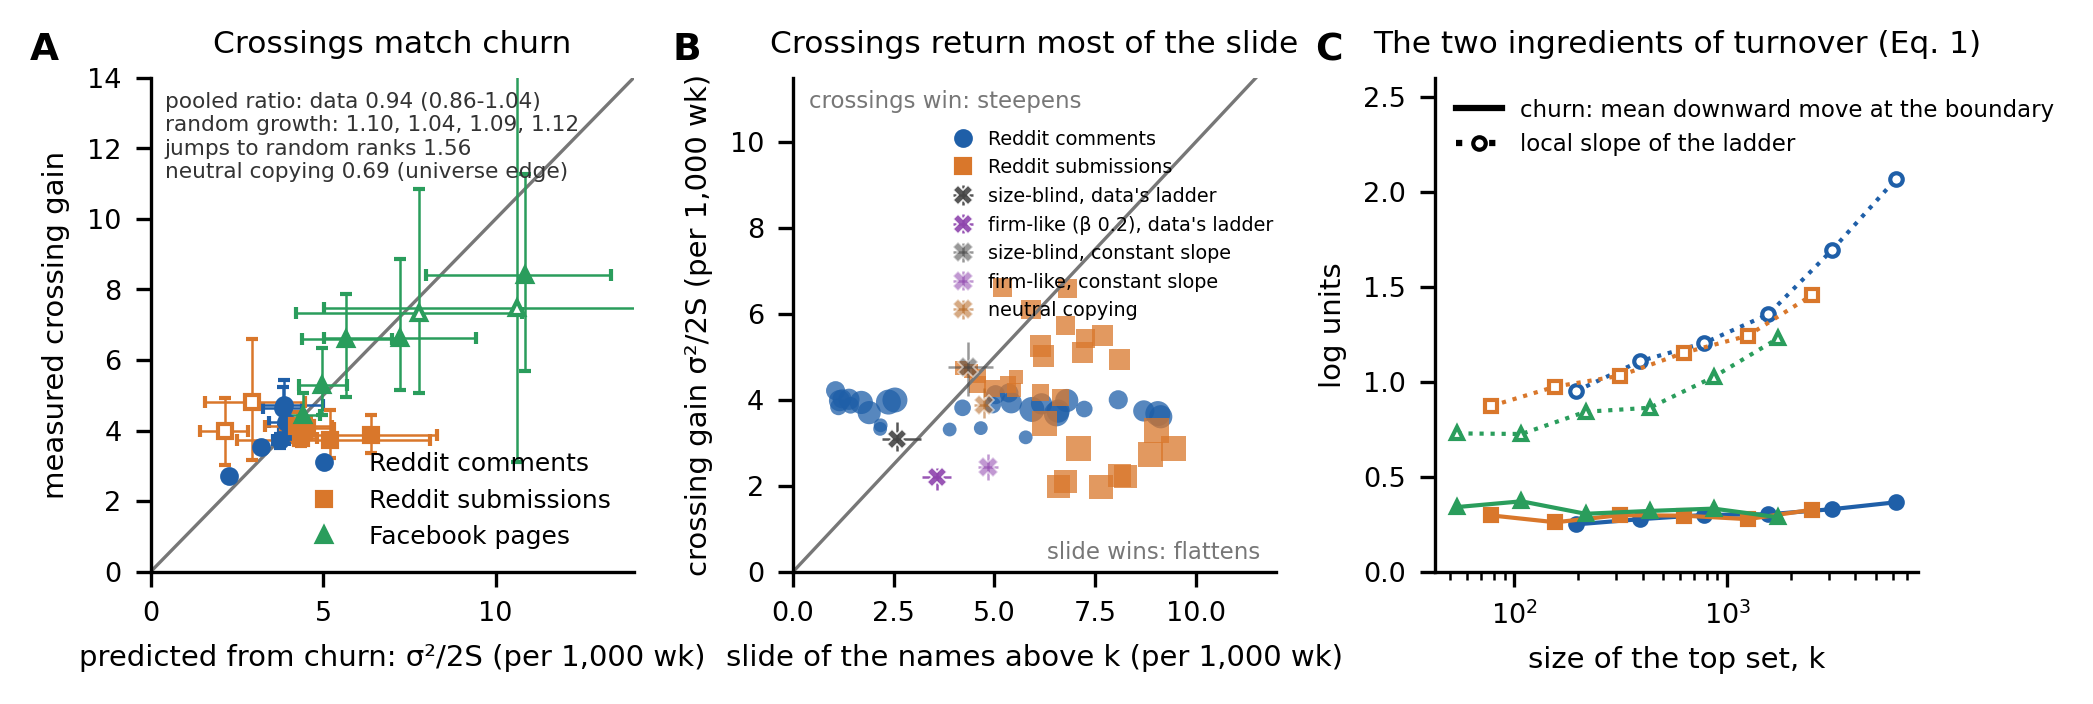
\includegraphics[width=\textwidth]{fig3_replenish}
\caption{What turnover returns. (\textit{A}) Measured lasting crossing gain at each cut-off $K/64\ldots K$ against Eq.~\ref{eq:crossing}, three ladders (5--95\% intervals; open symbols, boundary strata of $<150$ names); pooled ratios for the data and the simulated worlds (20 runs each) in the corner. (\textit{B}) Crossing gain $\sigma_k^2/(2S_k)$ against the slide of the names above $k$ (Reddit, 30 half-year-start intervals each; larger symbols are higher ranks), with the mean and 90\% range of each simulated world. On the diagonal the shape holds; below it, the hierarchy flattens toward its balance. (\textit{C}) The two ingredients of Eq.~\ref{eq:turnover} by cut-off: the mean downward move at the boundary (solid) and the local slope (dotted).}
\end{figure*}

The balance between the two terms says why the hierarchy is durable (Fig.~3\textit{B}). Crossings return 0.0040 a week on average against a slide of 0.0055, about three quarters. Because $c_k/\bar s_k = S^\ast_k/S_k$, this is the same statement as that the observed ladder is steeper than its own balance ($S^\ast_k/S_k$ = 0.72 on average) and is relaxing toward it; it is a description of the ladder's state, not of a mechanism, and every simulated world that starts steeper than its balance shows it (firm-like growth 0.51 from a ladder of constant slope and 0.62 from the data's ladder, neutral copying 0.82; 20 runs each), while driftless size-blind growth from the data's ladder steepens it (1.21). A positive slide is partly definitional too: measured against the re-selected universe, members of a top set lose ground even under driftless size-blind growth (0.0044 a week). What makes the hierarchy durable is the size of the two terms. Each is a fraction of a percent of the hierarchy's span a week, and they nearly cancel, so its shape relaxes over years---2 to 6 on the submissions head, 5 to 22 on comments---while a quarter of its leaders are replaced every year. The members turn over on the scale of the boundary crossings; the hierarchy changes on the scale of their small net imbalance. Without the crossing term the shape change is missed badly (root-mean-square error 0.0040 a week, worse than ``no change'' at 0.0029); with it the error is 0.0011. The variation across ranks and years comes from the slide: the crossing gain is close to constant across ranks, as Eq.~\ref{eq:crossing} implies when $\sigma^2/S$ is, and constant across years by construction, because lasting variance is estimated once per stratum (\textit{SI Appendix}).
%% law cells (half-year starts: c 0.0040, sbar 0.0055; rms 2.89 / 3.96 / 1.13 per 1,000 wk); R7 (c/s by world); §2z-bf; §2z-cp

\subsection*{Where the hierarchy comes from: a generative model}
These ingredients define a model, which we built and tested (\textit{Materials and Methods}; \textit{SI Appendix}). Each community has a lasting level $H_i$ that wanders with volatility that falls only weakly with size, under drift that depends on its rank,
\begin{equation}
H_i(t+1) = H_i(t) + g\big(r_i(t)\big) + \sigma(H_i)\,\eta_i(t),
\end{equation}
with $\sigma(H) = \sigma_0 e^{-\beta (H - H_0)}$, and its observed log activity is $H_i$ plus deviations that revert toward it at rank-dependent rates (taken from our earlier permanent--transitory model, whose own fixed home this replaces), a fast swing and observation noise. Communities leave at rank-dependent rates and are replaced at the bottom. The volatility parameters come from a structure function of each stratum's changes; the drift by rank is taken from the measured slides or solved to hold the training ladder. The lasting core has two scalars ($\sigma_0$, $\beta$) and the drift profile; the inherited parts are profiles by permanent rank on a grid of up to 60 ranks, each estimated from a declared moment, so the model has hundreds of numbers, none fitted to the statistics we test it on.

The model's lasting core shows where the hierarchy comes from (Fig.~4). Started from complete equality with the measured volatility and slides, it builds a hierarchy within about a decade (Fig.~4\textit{A}) whose steepness at each rank is $\sigma_k^2/(2\bar s_k)$, as the stationary identity requires (Fig.~4\textit{B}); started from the observed 2019 ladder, which is steeper, it relaxes toward the same steepness, and after 30 years the two runs agree within 5--16\% at every cut-off. Remove either ingredient and the hierarchy is not held (Fig.~4\textit{C}; 20 runs each): without volatility the slide flattens the head's shape by 61\% (comments) and 90\% (submissions) in 30 years, and without the slide volatility steepens it without limit ($+28\%$ and $+67\%$, still rising). The balance works over decades. Over two years neither removal moves the head by more than 0.3 log units a year, and on comments removing volatility at first slows the head's flattening, because the slide measured against the re-selected universe is itself partly produced by turnover (\textit{SI Appendix}). The balance the model reaches is flatter than the observed ladder at every rank, by 8--46\% (the 90\% bands of 20 runs exclude the observed slope at every cut-off except the head of submissions): the same fact as the three-quarter balance of Fig.~3\textit{B}, seen from the model.
%% §2z-dg A3; R3-C (flat start, 20 seeds); R6 (long30)

On held-out weeks the model forecasts the distribution of rank changes over 1 to 13 weeks no better than simpler models (Fig.~4\textit{D}): rolling-origin errors of 0.183 against 0.188 for the fixed-home model on four years of Reddit submissions, where carrying the training statistics forward does better (0.163), and 0.130 against 0.123 on comments, where removing its drift by rank lowers the error to 0.100. At these horizons the lasting process is close to invisible: fixed or wandering homes, with or without drift by rank, differ by at most 0.031. A first frozen version failed on the long submissions panel (0.246) through an error in its variance bookkeeping, corrected here (\textit{SI Appendix}); the corrected model over-disperses 13-week moves and its changes are too thin-tailed (excess kurtosis 2.9 against 22.1 on submissions). Fitted to 2019--20 and run forward, it forecasts one-year retention in 2021--22 with a mean absolute error across four cut-offs of 0.028 on submissions and 0.022 on comments, against 0.024 and 0.041 for the fixed-home model and 0.037 and 0.013 for carrying the previous year's retention forward; no model forecasts the fall of the submissions head (its share in the model's tracked universe was 0.51 in 2020 and 0.36 in 2022, against 0.53--0.54 forecast).
%% §2z-dg A5c (2x2), A6; R3-C; GATE_LEDGER

\begin{figure*}[tbp]\centering
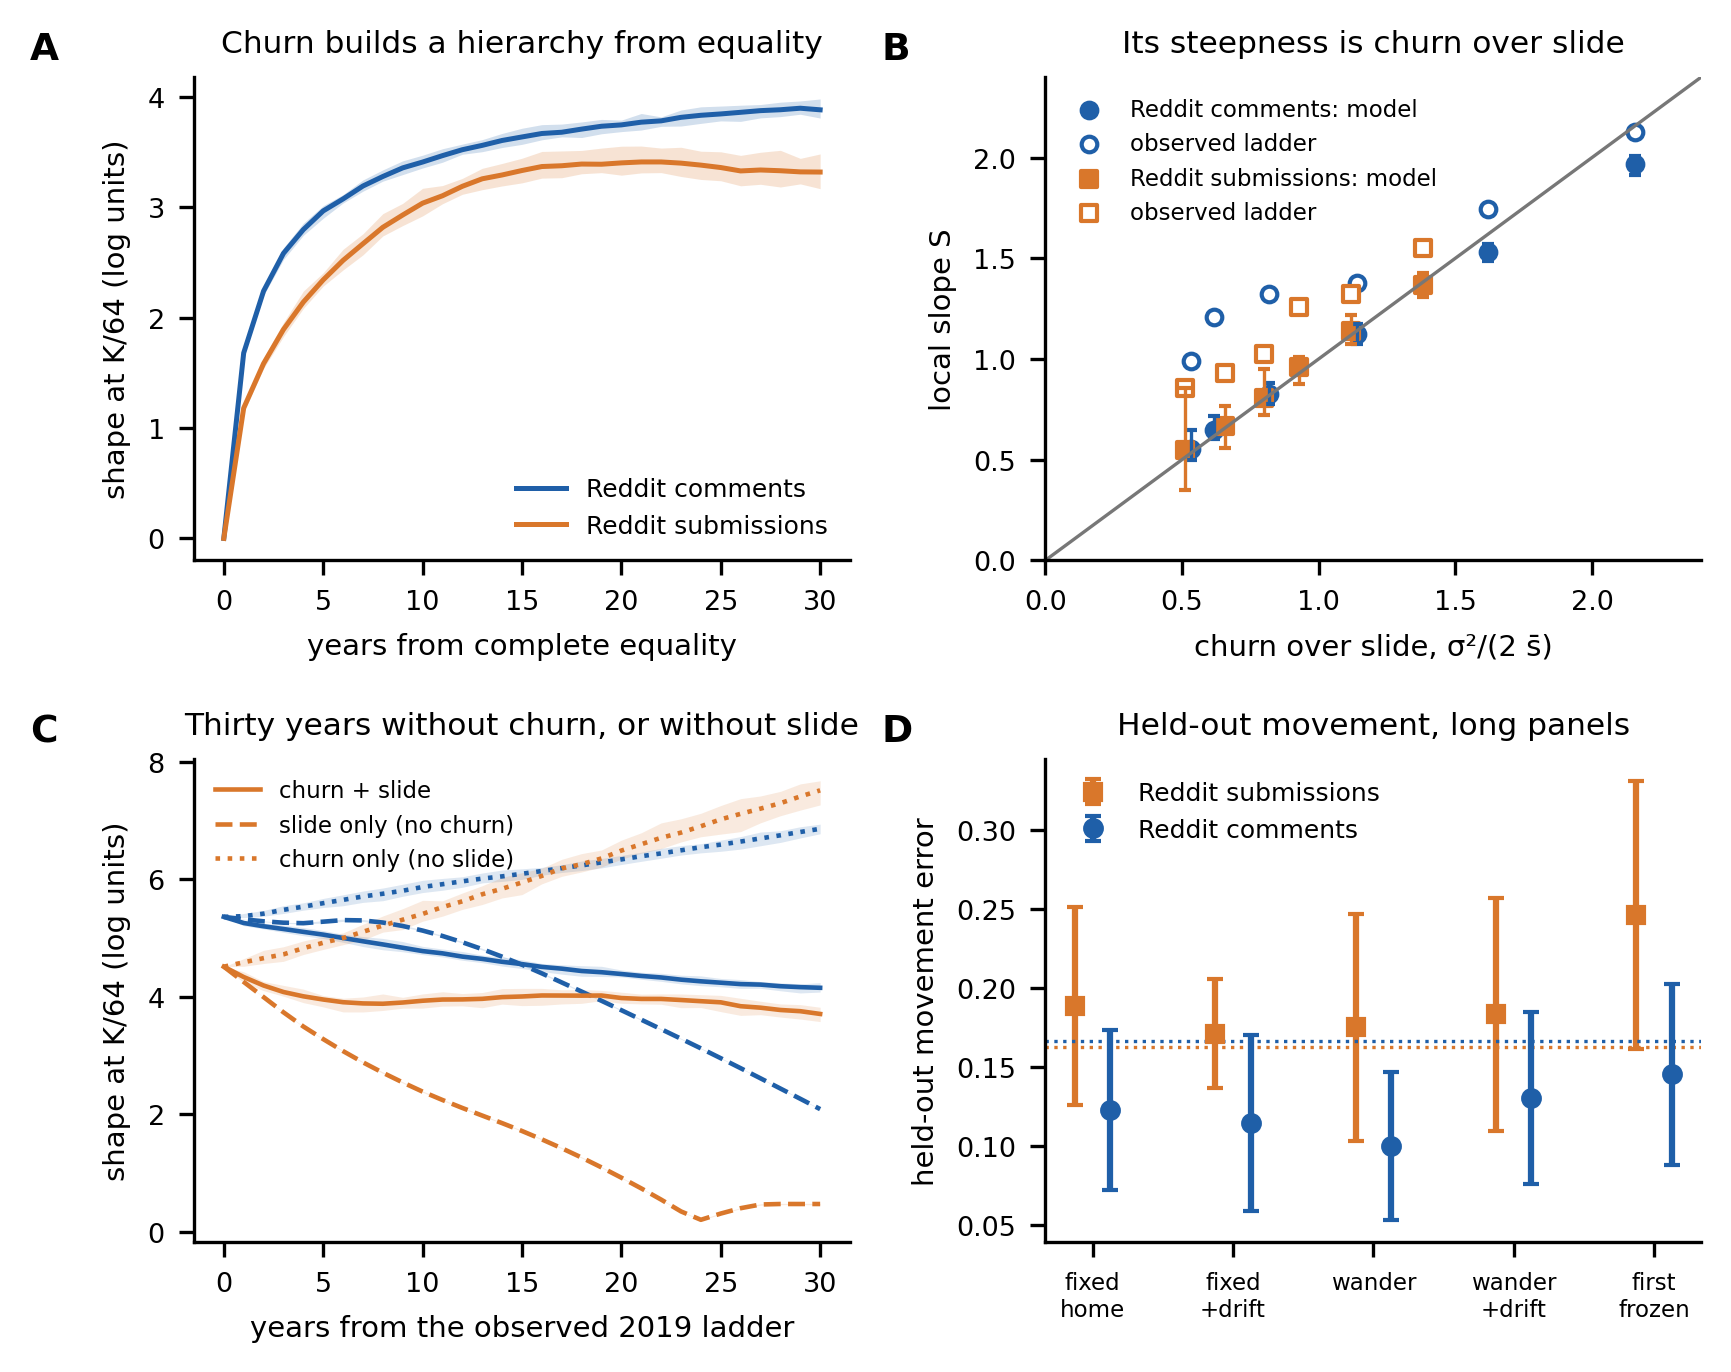
\includegraphics[width=0.70\textwidth]{fig4_model}
\caption{Where the hierarchy comes from. (\textit{A}) From complete equality, the model's lasting core with the measured volatility and slides builds a hierarchy (shape at $K/64$ by year; 20 runs, 90\% band). (\textit{B}) The local slope it reaches after 30 years (filled, 90\% band) against volatility over slide in the simulation, and the observed slopes (open). (\textit{C}) Thirty years from the observed 2019 ladder with volatility and slide (solid), the slide only (dashed) and volatility only (dotted); blue, comments; orange, submissions; 20 runs, 90\% bands. (\textit{D}) Held-out movement error on the four-year panels (mean $\pm$ sd over five origins; dotted, carrying the training statistics forward) for a fixed home (the earlier model), a fixed home sliding by rank, a wandering home, a wandering home with drift by rank (the model), and the first frozen version.}
\end{figure*}
\subsection*{What random growth lacks: persistent decline}
One feature of the data appears in no simulated world. The correlation of consecutive changes of a community's annual mean activity is $+0.32$ to $+0.45$ on Reddit, but averaging a random walk over blocks alone produces about $+0.24$ \cite{working1960}. We therefore correlate changes that share no weeks: the change between two 13-week windows a year apart, against the same change starting 13 or 26 weeks after the first ends. Any process with independent increments plus short-memory noise gives zero or less, and every simulated world gives $-0.02$ to $-0.10$ (20 runs each). On Reddit the correlation is $+0.14$ to $+0.20$ on both ladders, positive at every origin and still $+0.14$ with a half-year gap; on Facebook pages it is negative at every gap (Fig.~5\textit{A}). Neither the surge of Reddit activity in early 2020, which every such annual comparison spans, nor the change in how the archive captured Reddit in July 2021 accounts for it alone: with 4-week windows, comparisons that begin after the surge give $+0.13$ to $+0.16$, and comparisons that end before the capture change give $+0.07$ to $+0.14$, against $-0.02$ to $-0.16$ in the simulated worlds (post hoc; each set rests on one to four overlapping starts). No comparison in these data excludes both.
%% §2z-df; R3-A; R4, R4b (persistence_post2020.py)

Persistence means that communities differ in their mean growth for a year or more, as types do in models of income dynamics \cite{gllm2016,guvenen2009}; it is also the source of the positive composition term in the crossing statistic on Reddit. It is familiar elsewhere: the serial correlation of firm growth depends on size \cite{coad2007}, the growth of online groups on how their members are connected \cite{kairam2012}, and different early features predict the growth, retention and survival of Reddit communities \cite{cunha2019}, which also compete with and support one another \cite{teblunthuis2022}. The persistence here is in participation. The number of posts or comments carries it ($+0.13$ to $+0.19$), the engagement each earns little ($+0.02$ to $+0.07$). It is concentrated in decline: among communities whose activity fell in the first year the correlation is $+0.16$ to $+0.19$, among those whose activity rose $0.00$ to $+0.03$, and the lowest fifth of first-year changes is followed by the lowest second-year changes (mean rank 0.40--0.41, against 0.52--0.54 for the highest fifth). Its origin differs by ladder. On submissions it is heterogeneous exposure to a platform-wide trend: removing each community's loading on the platform's total activity, estimated from weekly co-movement in 2019 alone, removes it (from $+0.11$ to between $-0.03$ and $+0.01$ at a half-year gap, on matched origins), and it fades within a year---Gomez's aggregate-risk term \cite{gomez2023}. On comments it survives that adjustment and is still $+0.11$ a year later. Measured over 26 weeks from December 2020, the horizon available for Facebook, Reddit's persistence is weak ($-0.04$ to $+0.08$), so the platform contrast rests on the annual horizon. Choosing the universe from the first half-year alone changes these statistics by less than 0.01, and counts of posts and comments, which carry the persistence, are less exposed to capture effects than karma.
%% §2z-dg A4; R3-D

\begin{figure*}[tbp]\centering
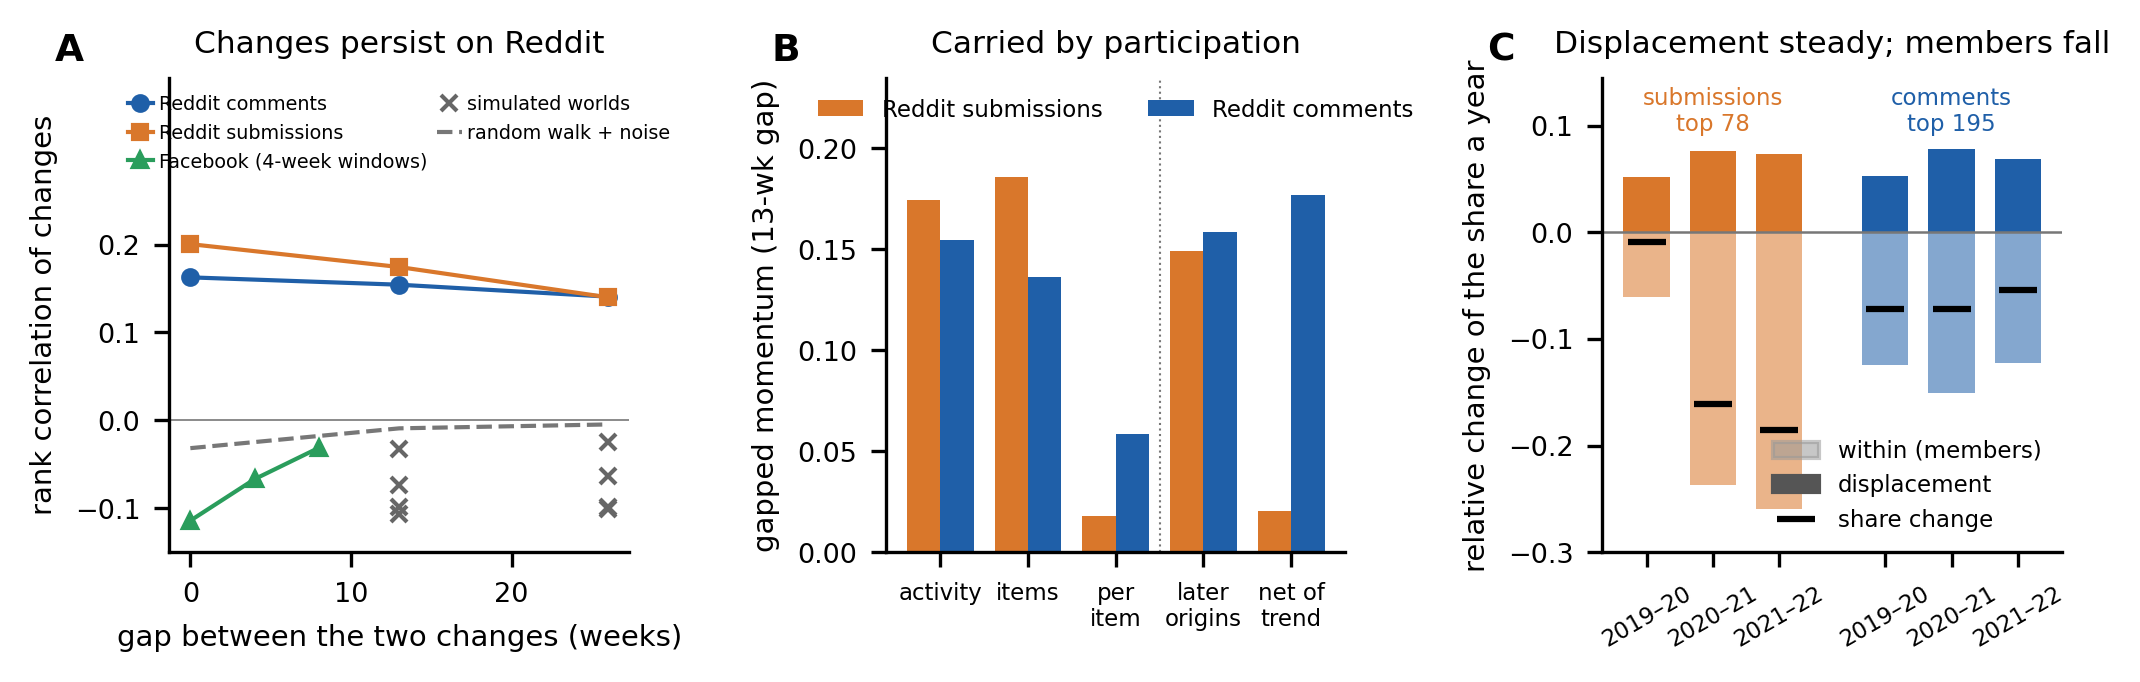
\includegraphics[width=\textwidth]{fig5_tipping}
\caption{What random growth lacks. (\textit{A}) Rank correlation between changes that share no weeks (13-week windows a year apart; Facebook, 4-week windows half a year apart) against the gap between them; dashed, a simulated size-blind random walk with a short-memory swing and noise; crosses, the four simulated worlds of Fig.~2. (\textit{B}) The same statistic at a 13-week gap for activity, for the number of items and for activity per item (all origins), and for activity before and after removing each community's loading on the platform's total activity (origins after the first year, where the loadings are estimated). (\textit{C}) Annual relative change of the arithmetic share of the head (bars: within term, light; displacement, dark; dash: the share's change).}
\end{figure*}

Decline at the head is what moved concentration, and it came through participation. In Gomez's exact decomposition of the arithmetic shares (Fig.~5\textit{C}), displacement added $+0.04$ to $+0.08$ of each top set's share every year---a reordering gain, non-negative by construction---while the members' own growth relative to the total subtracted $-0.04$ to $-0.26$. In 2019--20, when the submissions head's share held steady, the members' term ($-0.06$) was the size expected from selecting each year's leaders on noise, which a size-blind world started from the data's ladder puts at $-0.05$; in 2020--22 it was $-0.24$ and $-0.26$ a year, and the share fell by a third. Choosing each cohort a year earlier, so that selection uses none of the activity in the change, makes the members' term larger ($-0.25$ and $-0.31$). Split exactly into its share of items and the engagement each item earns, the head's fall was in posting: its share of the top 5,000's submissions fell from 22\% to 9\%, while the karma per post it earned rose from 2.3 to 3.9 times the top 5,000's (comments: share of comments 41\% to 31\%, karma per comment 1.48 to 1.61 times). That is the component that carries persistence, though we have not shown that the communities whose declines persist are the head's decliners. Gomez's general prediction of displacement is within a factor of 1.5 of the measured term at the head of both ladders (\textit{SI Appendix}).
%% §2z-dg A8; R3-E; R7 (gomez_r7_prior.py; size-blind world baseline); R8 (head_components.py)

\section*{Discussion}
The occupants of an attention hierarchy change much faster than the hierarchy does, and random-growth theory says why. The hierarchy is a balance between the volatility that spreads communities apart and the relative decline that pulls the leaders back. Built from the measured ingredients, it forms from equality, collapses without the volatility and steepens without limit without the decline; and it changes slowly because what members lose and what newcomers bring are each small against its span and nearly cancel. Constant turnover is therefore not in tension with a durable hierarchy: the crossings that replace its members are what hold its shape against their decline. Much of this is automatic in random growth; the contribution is to measure it rank by rank, for named units whose movement is mostly passing, and to separate what is automatic from what is not. Two features are not automatic. Lasting volatility falls with size less steeply than for firms. And participation, unlike a random walk, persists, above all in decline, and it is through participation that the leaders of Reddit submissions lost a third of their share.

These findings bear on entrenchment and on platform design. A leading community holds its rank because the gap below it is wide, not because its activity is steady: the largest communities of both Reddit ladders kept rank one while losing more than half of their share. The order in which top sets turn over is set by the hierarchy's shape, so a change that flattens the head exposes its members, whatever their size. A change in how a platform distributes attention acts on the balance through the relative decline of those above each rank, and because the hierarchy relaxes over years to decades, its effect on concentration can unfold long after the change is made.

The limits are those of the data. All results are from development data examined many times, and several analyses are post hoc, which we label (\textit{SI Appendix}). The units are karma and interactions, measures of engaged activity rather than views; item counts measure posting and commenting, not participants. The size range is two to three decades, and the size exponent depends on the estimator. The submissions shortfall of crossings at ranks 300--600 is unexplained. Persistence holds in comparisons that exclude the 2020 surge and in comparisons that exclude the archive's July 2021 capture change, but no comparison in these data excludes both, and other capture effects are not audited. The model's lasting core reaches its balance over decades, longer than any record here. We have written tests of the main claims on 2023--2024 Reddit data held sealed for the purpose---the boundary relation in period and a year ahead, persistence, the size exponent and the model's held-out movement---into a protocol that is to be adopted before those data are opened.

\matmethods{
\subsection*{Data}
Reddit ladders are built from the Pushshift archive of comments and submissions \cite{baumgartner2020}: for each community and day, comment karma and submission karma (negative daily values set to zero), summed to weeks, December 2018 to December 2022. Facebook ladders are weekly interactions of public Facebook Pages from CrowdTangle \cite{crowdtangle}, restricted to the period November 2020 to June 2022 in which coverage was stable, with flagged days excluded. Each ladder is a top-$K$ universe (Reddit comments $K$ = 12,500, submissions 5,000, Facebook 3,500) with membership penalised for absence; communities ever ranked inside $4K$ in a week are tracked. Log activity is $x = \log(1 + \text{activity})$. Arithmetic shares are the year's activity of the top $k$ by total over that of the top $K$. All contact with the data is logged; a 2023--2024 Reddit extension and a Wikipedia ladder are held sealed.

\subsection*{Cohorts, blocks and simulated worlds}
Blocks are non-overlapping, of 52 weeks (Facebook 13 or 26), aligned to the end of each panel; a block level requires presence in 90\% of its weeks. Permanent rank is a community's mean weekly rank over a fixed block, absences counted at that week's floor. Cohorts are fixed on a block disjoint from those they are measured on. The simulated worlds run 212 weeks with $K$ = 5,000, 20 runs each, and every statistic is computed by the same code in data and simulations (\textit{SI Appendix}). Constant-slope worlds start from a Zipf ladder with passing swings; neutral copying draws 1.5 million items a week from last week's distribution with innovation rate 0.003; calibrated worlds are the generative model estimated on Reddit submissions, started from the data's 2019 ladder with a planted $\beta$ and no drift by rank; the model world holds its training ladder, which is then an input. 

\subsection*{Estimators}
$\beta$ is minus the slope of log standard deviation of one-year change on mean log size across seven octave strata of permanent rank; intervals resample communities. Turnover is one minus the overlap of the top $k$ by block level in consecutive blocks. Lasting variance at rank $k$ is the growth with spacing of the variance of a cohort's changes (blocks one to three years apart). Crossings are the reordering gain of the top $k$ differenced between spacings of two and four half-years; the result is the lasting crossing gain plus a composition term. The slide is the mean change of a cohort's members above $k$ against the mean of the universe. Pooled ratios are geometric means over cut-offs $K/16 \ldots K$; joint intervals give each community one Poisson weight shared by the variance and every start, and resample the starts.

\subsection*{The generative model and its tests}
The model (\texttt{rankdiff\_rdm.py}) is estimated from a structure function of each stratum's changes ($\sigma_0$, $\beta$), the reverting deviations, fast swing and noise of the earlier model, and exit rates by rank. Held-out movement is scored by a rolling-origin test: five origins; a cohort of the 200 top communities at each origin, simulated 20 times from the filtered state; the median absolute rank change at 1, 4 and 13 weeks, its first autocorrelation and collision rates at the top, each as relative error; an observation-noise scale is recalibrated on each training window. Persistence of the training-window statistics is the baseline. Every evaluation is logged with its outcome.

\subsection*{Registration and AI use}
Expected outcomes were written down before each analysis, and committed before it except where the record notes otherwise; post hoc analyses are labelled, and failed expectations are reported with passed ones (\textit{SI Appendix}). The analyses, code and drafts were produced with AI coding agents (Anthropic Claude Opus 5.5; OpenAI Codex, gpt-6-astra) under the authors' direction, with four rounds of review by further models; every number was checked against saved outputs.

\subsection*{Data, materials, and software availability}
%% Sources and precedents: llm_fitting/runs/2026-10-18_pnas_push/DATA_AVAILABILITY_NOTES.md; owner decisions MODEL_STATUS §2z-dh §§9--10
Code, every analysis output and the analysis record are deposited in a public repository \todo{URL and DOI of a frozen snapshot}. Reddit data are from the Pushshift archive of Reddit comments and submissions \cite{baumgartner2020}, monthly files for December 2018 to December 2022 \todo{acquisition source and date}; we do not redistribute them or the community-level weekly panels built from them. The deposit contains the code that builds the panels from those files and every result, including results for named communities; no analysis uses user-level data. Facebook and Instagram data were obtained from CrowdTangle, a public insights tool owned and operated by Facebook (now Meta), which tracked interactions on public content and did not include paid advertising or private accounts \cite{crowdtangle}; CrowdTangle was discontinued on 14 August 2024. Its terms for researchers do not permit sharing its data outside the research team, so we deposit neither the CrowdTangle exports nor the weekly Page-level series built from them; every Facebook and Instagram result reported here is an aggregate over Pages. As those terms permit, the deposit lists the IDs of the Facebook Pages in the study universe \todo{owner: confirm publishing Page IDs}, so that researchers with access to Meta Content Library can locate them; because that library uses its own identifiers and current engagement, a rebuilt panel will approximate rather than reproduce ours. Editors and reviewers can have any deposited result regenerated from the authors' copies of the data on request; the data themselves are not transferred.
}
\showmatmethods{}

\acknow{\todo{Acknowledgements.}}
\showacknow{}

\bibliography{references}

\end{document}
